\begin{frame}{Thermalization Problem}
  \begin{columns}
    \column{0.5\textwidth}
    \vspace{.5cm}
    \begin{itemize}
      \item Neutral helium particles with two populations with two different initial temperatures $\alpha$ and $\beta$.
      \begin{itemize}
        \item $T_\alpha(0) = 1,000$ $\text{\fontfamily{STIX2Text-TLF}\selectfont K}$.
        \item $T_\beta(0) = 100$ $\text{\fontfamily{STIX2Text-TLF}\selectfont K}$.
      \end{itemize}
        \item Number density $n_0 = 10^{25}$ $\text{\fontfamily{STIX2Text-TLF}\selectfont m}^{-3}$.
        \item Interpopulation cross section $\sigma_0 = 10^{-18}$ $\text{\fontfamily{STIX2Text-TLF}\selectfont m}^{2}$.
        \item Intrapopulation cross section $\sigma_1 = 100 \;\sigma_0$.
    \end{itemize}
    \column{0.5\textwidth}
      \vspace{0.5cm}
      \begin{align*}
        \text{Ar}_\alpha + \text{Ar}_\alpha \to \text{Ar}_\alpha + \text{Ar}_\alpha \\
        \text{Ar}_\beta + \text{Ar}_\beta \to \text{Ar}_\beta + \text{Ar}_\beta \\
        \text{Ar}_\alpha + \text{Ar}_\beta \to \text{Ar}_\alpha + \text{Ar}_\beta \\
      \end{align*}
      \pause
      \vspace{-.75cm}
      \begin{align*}
        T_\alpha(t) = 550 + 450 e^{-\frac{ 4 }{ 3 }\nu_{\alpha, \beta} t}\\
        T_\beta(t) = 550 - 450 e^{-\frac{ 4 }{ 3 }\nu_{\alpha, \beta} t}\\
        \nu_{\alpha,\beta} =
        \frac{
          m_{\alpha} m_\beta
        }{
          \left( m_\alpha + m_\beta \right)^2
        }
        3 n_0 \sigma_0
      \end{align*}
  \end{columns}
\end{frame}

\begin{frame}{Thermalization Results}
  \begin{columns}
    \column{0.5\textwidth}
      \begin{itemize}
        \item Repeated $10$ times with a different seed value for the pseudorandom number generators.
        \item Simulated on a $4\times4$ grid where $x, y \in [-1, 1] \times 10^{-5}$ $\text{\fontfamily{STIX2Text-TLF}\selectfont m}^{2}$. with reflective boundary conditions.
        \item Time step $\Delta t = 0.1$ $\text{\fontfamily{STIX2Text-TLF}\selectfont ns}$.
        \item Particles per element: $N_p = 1,000$ for $\alpha$ and $\beta$.
      \end{itemize}
    \column{0.5\textwidth}
    \pause
    \vspace{1cm}
    \begin{figure}[H]
      \centering
      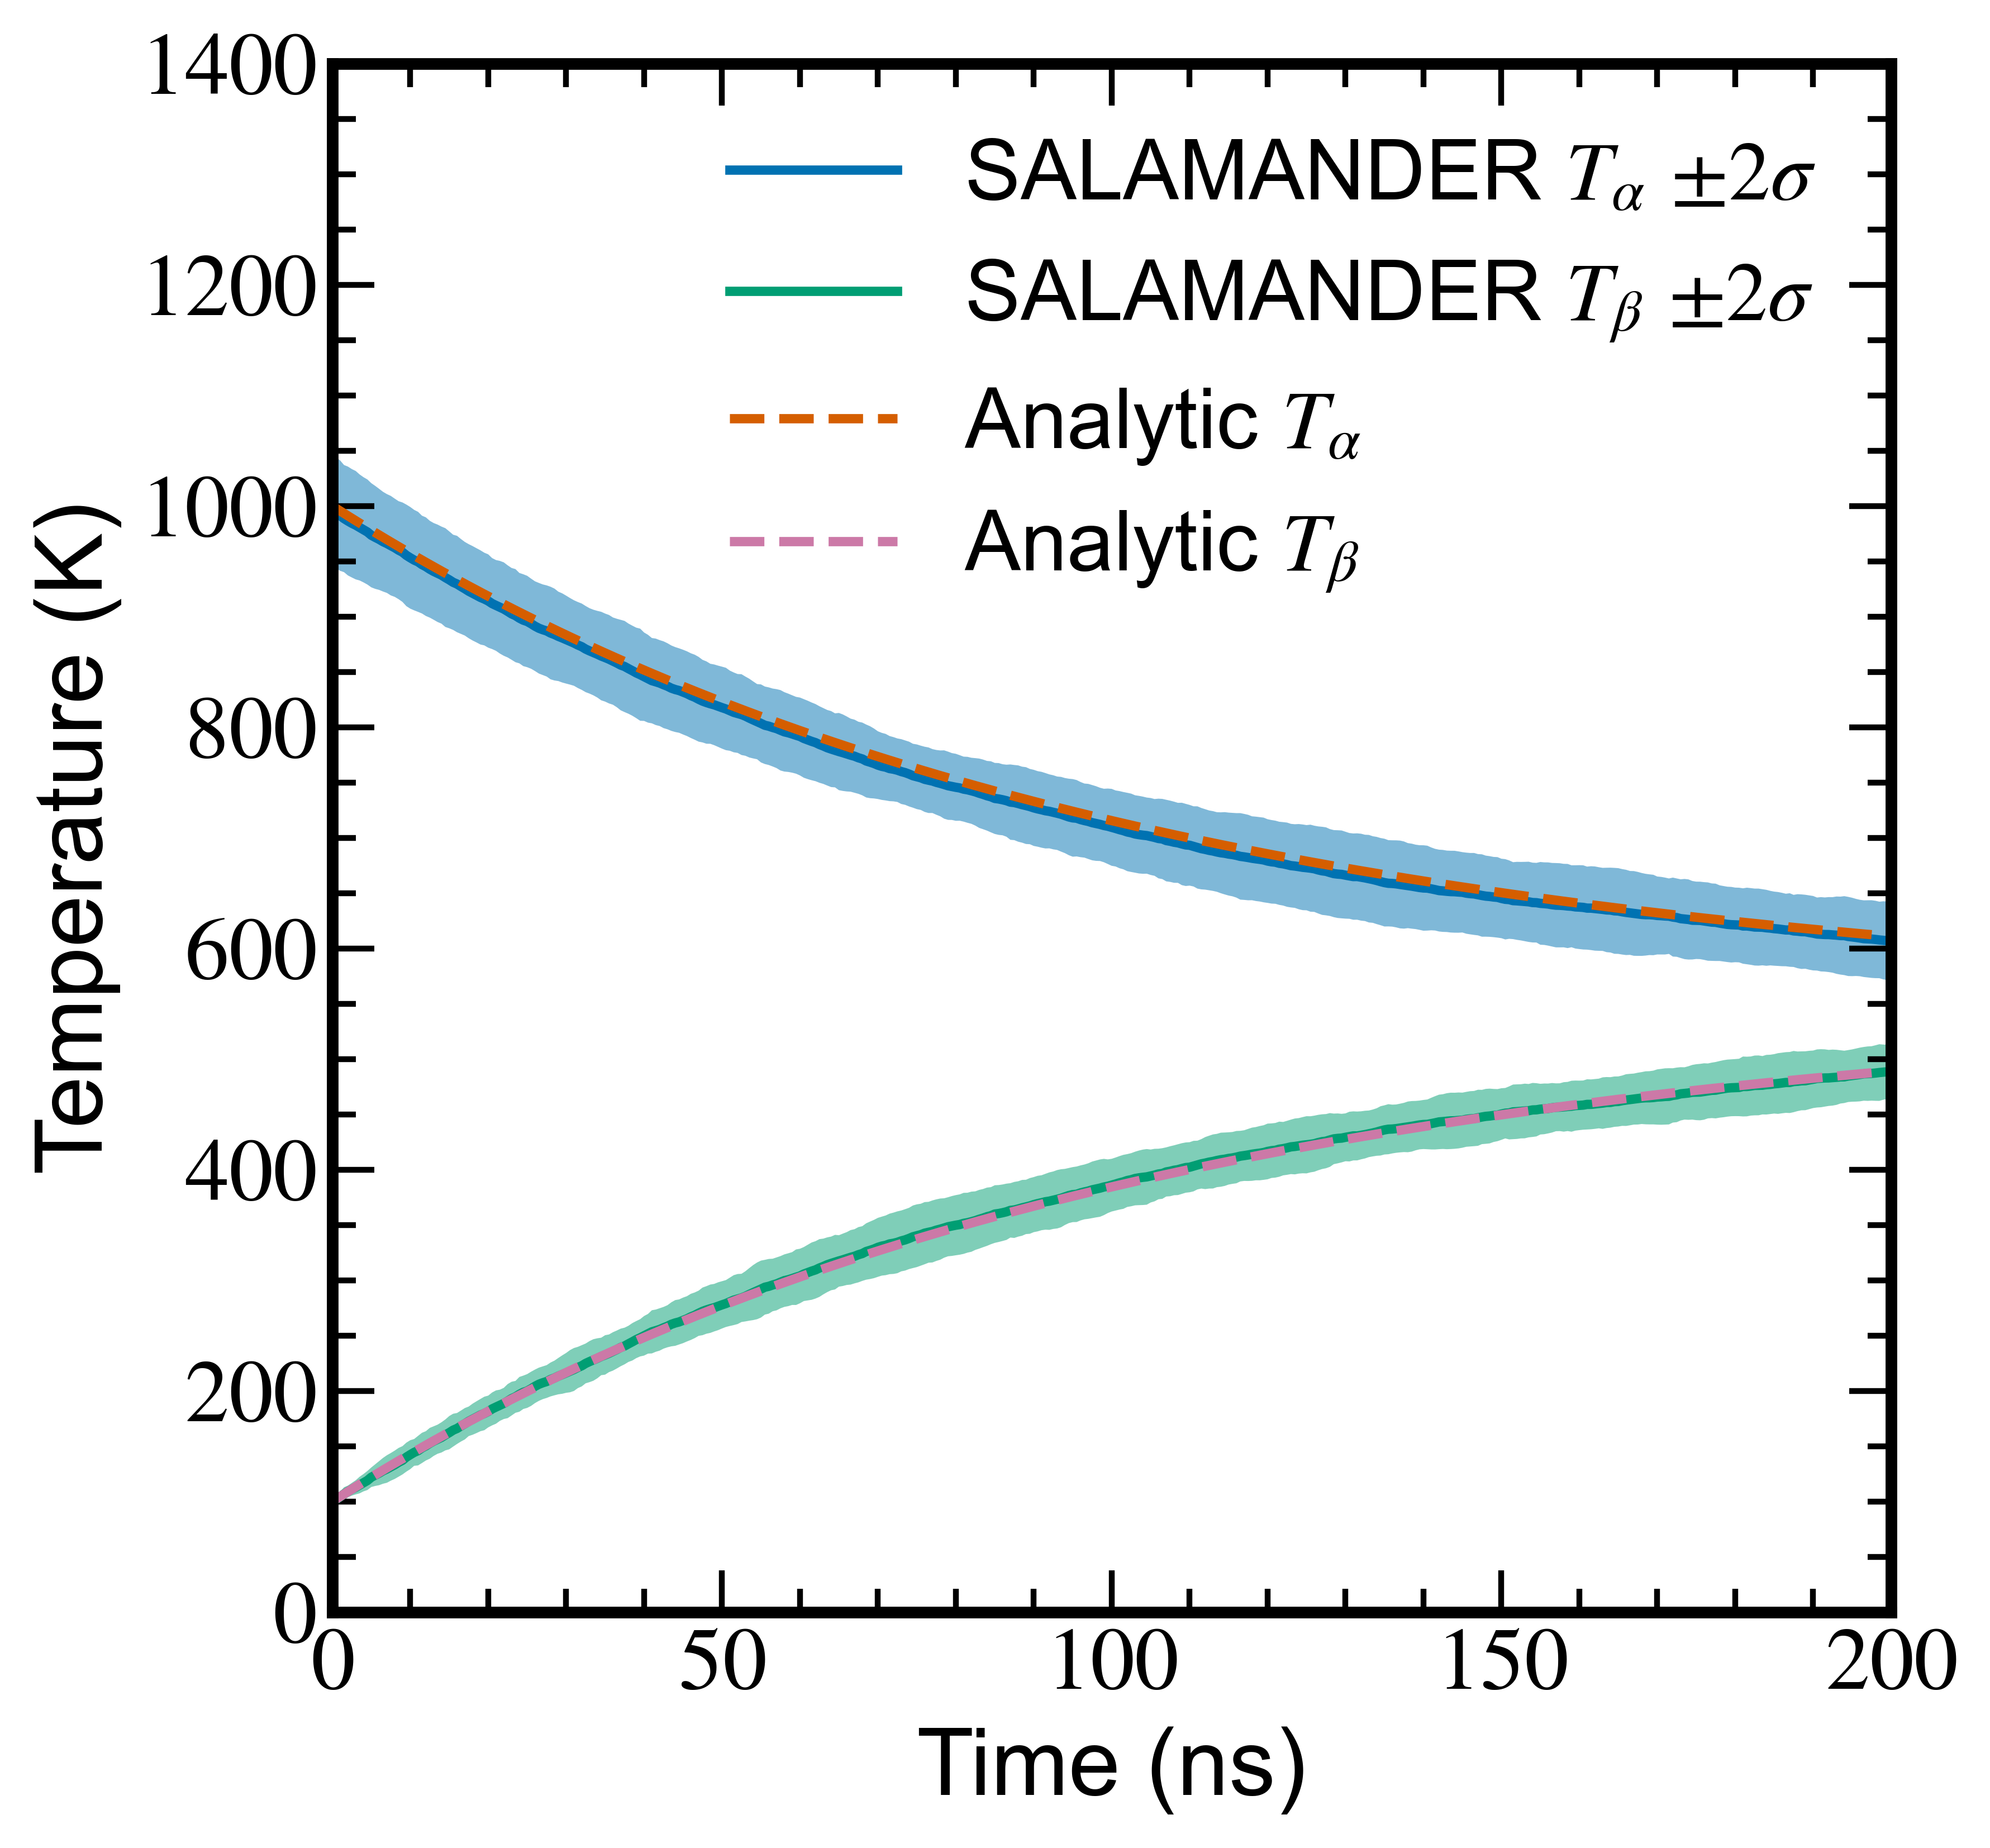
\includegraphics[width=0.9\textwidth]{figs/theramlization.png}
    \end{figure}
  \end{columns}
\end{frame}

\begin{frame}{Thermalization Distribution Evolution}
  \vspace{1cm}
  \begin{columns}
    \column{0.5\textwidth}
%    \animategraphics[autoplay,loop,controls,height=0.75\textheight]{30}{gifs/alpha_frames/frame.}{0}{180}
    \animategraphics[autoplay,loop,height=0.75\textheight]{30}{gifs/alpha_frames/frame.}{0}{180}
    \column{0.5\textwidth}
%   \animategraphics[autoplay,loop,controls,height=0.75\textheight]{30}{gifs/beta_frames/frame.}{0}{180}
    \animategraphics[autoplay,loop,height=0.75\textheight]{30}{gifs/beta_frames/frame.}{0}{180}
  \end{columns}
\end{frame}

